\documentclass[review]{elsarticle}

\usepackage{multirow}
\usepackage{lineno}
\usepackage{xspace}
\usepackage{threeparttable}
\usepackage{subfig}
\modulolinenumbers[5]

\journal{Progress in Nuclear Energy}

%% `Elsevier LaTeX' style
\bibliographystyle{elsarticle-num}
%%%%%%%%%%%%%%%%%%%%%%%

%%%% packages and definitions (optional)
\usepackage{placeins}
\usepackage{booktabs} % nice rules (thick lines) for tables
\usepackage{microtype} % improves typography for PDF
\usepackage{hhline}
\usepackage{amsmath}
\usepackage{subfig}

%\usepackage{graphicx}
%\usepackage{caption}
%\usepackage{subcaption}

\usepackage{booktabs}
\usepackage{threeparttable, tablefootnote}
\graphicspath{ {../images/} {../images/isos/} {../images/err/}  }
\usepackage{tabularx}
\newcolumntype{b}{>{\hsize=1.0\hsize}X}
\newcolumntype{s}{>{\hsize=.5\hsize}X}
\newcolumntype{m}{>{\hsize=.75\hsize}X}
\newcolumntype{x}{>{\hsize=.25\hsize}X}

\newcommand{\Cyclus}{\textsc{Cyclus}\xspace}%
\newcommand{\Cycamore}{\textsc{Cycamore}\xspace}%

% tikz %
\usepackage{tikz}
\usetikzlibrary{positioning, arrows, decorations, shapes}

\usetikzlibrary{shapes.geometric,arrows}
\tikzstyle{process} = [rectangle, rounded corners, minimum width=3cm, minimum height=1cm,text centered, draw=black, fill=blue!30]
\tikzstyle{object} = [ellipse, rounded corners, minimum width=3cm, minimum height=1cm,text centered, draw=black, fill=green!30]
\tikzstyle{arrow} = [thick,->,>=stealth]

% hyperref %
\usepackage[hidelinks]{hyperref}
% after hyperref %
\usepackage{cleveref}
\usepackage{datatool}
\usepackage[acronym,toc]{glossaries}
%\newacronym{<++>}{<++>}{<++>}
\newacronym[longplural={metric tons of heavy metal}]{MTHM}{MTHM}{metric ton of heavy metal}
\newacronym{ABM}{ABM}{agent-based modeling}
\newacronym{ACDIS}{ACDIS}{Program in Arms Control \& Domestic and International Security}
\newacronym{ADS}{ADS}{Accelerator-Driven System}
\newacronym{AFCI}{AFCI}{Advanced Fuel Cycles Initiative}
\newacronym{AHTR}{AHTR}{Advanced High Temperature Reactor}
\newacronym{ANDRA}{ANDRA}{Agence Nationale pour la gestion des D\'echets RAdioactifs, the French National Agency for Radioactive Waste Management}
\newacronym{ANL}{ANL}{Argonne National Laboratory}
\newacronym{ANS}{ANS}{American Nuclear Society}
\newacronym{API}{API}{application programming interface}
\newacronym{ARE}{ARE}{Aircraft Reactor Experiment}
\newacronym{ARFC}{ARFC}{Advanced Reactors and Fuel Cycles}
\newacronym{ASME}{ASME}{American Society of Mechanical Engineers}
\newacronym{ASTRID}{ASTRID}{Advanced Sodium Technological Reactor for Industrial Demonstration}
\newacronym{ATWS}{ATWS}{Anticipated Transient Without Scram}
\newacronym{BDBE}{BDBE}{Beyond Design Basis Event}
\newacronym{BIDS}{BIDS}{Berkeley Institute for Data Science}
\newacronym{BWR}{BWR}{Boiling Water Reactor}
\newacronym{CAFCA}{CAFCA}{ Code for Advanced Fuel Cycles Assessment }
\newacronym{CDTN}{CDTN}{Centro de Desenvolvimento da Tecnologia Nuclear}
\newacronym{CEA}{CEA}{Commissariat \`a l'\'Energie Atomique et aux \'Energies Alternatives}
\newacronym{CI}{CI}{continuous integration}
\newacronym{CNEN}{CNEN}{Comiss\~{a}o Nacional de Energia Nuclear}
\newacronym{CNERG}{CNERG}{Computational Nuclear Engineering Research Group}
\newacronym{COSI}{COSI}{Commelini-Sicard}
\newacronym{COTS}{COTS}{commercial, off-the-shelf}
\newacronym{CSNF}{CSNF}{commercial spent nuclear fuel}
\newacronym{CTAH}{CTAHs}{Coiled Tube Air Heaters}
\newacronym{CUBIT}{CUBIT}{CUBIT Geometry and Mesh Generation Toolkit}
\newacronym{CURIE}{CURIE}{Centralized Used Fuel Resource for Information Exchange}
\newacronym{DAG}{DAG}{directed acyclic graph}
\newacronym{DANESS}{DANESS}{Dynamic Analysis of Nuclear Energy System Strategies}
\newacronym{DBE}{DBE}{Design Basis Event}
\newacronym{DESAE}{DESAE}{Dynamic Analysis of Nuclear Energy Systems Strategies}
\newacronym{DHS}{DHS}{Department of Homeland Security}
\newacronym{DOE}{DOE}{Department of Energy}
\newacronym{DRACS}{DRACS}{Direct Reactor Auxiliary Cooling System}
\newacronym{DRE}{DRE}{dynamic resource exchange}
\newacronym{DSNF}{DSNF}{DOE spent nuclear fuel}
\newacronym{DYMOND}{DYMOND}{Dynamic Model of Nuclear Development }
\newacronym{EBS}{EBS}{Engineered Barrier System}
\newacronym{EDF}{EDF}{Électricité de France}
\newacronym{EDZ}{EDZ}{Excavation Disturbed Zone}
\newacronym{EIA}{EIA}{U.S. Energy Information Administration}
\newacronym{EPA}{EPA}{Environmental Protection Agency}
\newacronym{EPR}{EPR}{European Pressurized Reactor}
\newacronym{EP}{EP}{Engineering Physics}
\newacronym{EU}{EU}{European Union}
\newacronym{FCO}{FCO}{Fuel Cycle Options}
\newacronym{FCT}{FCT}{Fuel Cycle Technology}
\newacronym{FEHM}{FEHM}{Finite Element Heat and Mass Transfer}
\newacronym{FEPs}{FEPs}{Features, Events, and Processes}
\newacronym{FHR}{FHR}{Fluoride-Salt-Cooled High-Temperature Reactor}
\newacronym{FLiBe}{FLiBe}{Fluoride-Lithium-Beryllium}
\newacronym{FP}{FP}{Fission Products}
\newacronym{GDSE}{GDSE}{Generic Disposal System Environment}
\newacronym{GDSM}{GDSM}{Generic Disposal System Model}
\newacronym{GENIUSv1}{GENIUSv1}{Global Evaluation of Nuclear Infrastructure Utilization Scenarios, Version 1}
\newacronym{GENIUSv2}{GENIUSv2}{Global Evaluation of Nuclear Infrastructure Utilization Scenarios, Version 2}
\newacronym{GENIUS}{GENIUS}{Global Evaluation of Nuclear Infrastructure Utilization Scenarios}
\newacronym{GPAM}{GPAM}{Generic Performance Assessment Model}
\newacronym{GRSAC}{GRSAC}{Graphite Reactor Severe Accident Code}
\newacronym{GUI}{GUI}{graphical user interface}
\newacronym{HLW}{HLW}{high level waste}
\newacronym{HPC}{HPC}{high-performance computing}
\newacronym{HTC}{HTC}{high-throughput computing}
\newacronym{HTGR}{HTGR}{High Temperature Gas-Cooled Reactor}
\newacronym{IAEA}{IAEA}{International Atomic Energy Agency}
\newacronym{IEMA}{IEMA}{Illinois Emergency Mangament Agency}
\newacronym{IHLRWM}{IHLRWM}{International High Level Radioactive Waste Management}
\newacronym{INL}{INL}{Idaho National Laboratory}
\newacronym{IPRR1}{IRP-R1}{Instituto de Pesquisas Radioativas Reator 1}
\newacronym{IRP}{IRP}{Integrated Research Project}
\newacronym{ISFSI}{ISFSI}{Independent Spent Fuel Storage Installation}
\newacronym{ISRG}{ISRG}{Independent Student Research Group}
\newacronym{JFNK}{JFNK}{Jacobian-Free Newton Krylov}
\newacronym{LANL}{LANL}{Los Alamos National Laboratory}
\newacronym{LBNL}{LBNL}{Lawrence Berkeley National Laboratory}
\newacronym{LCOE}{LCOE}{levelized cost of electricity}
\newacronym{LDRD}{LDRD}{laboratory directed research and development}
\newacronym{LFR}{LFR}{Lead-Cooled Fast Reactor}
\newacronym{LLNL}{LLNL}{Lawrence Livermore National Laboratory}
\newacronym{LMFBR}{LMFBR}{Liquid Metal Fast Breeder Reactor}
\newacronym{LOFC}{LOFC}{Loss of Forced Cooling}
\newacronym{LOHS}{LOHS}{Loss of Heat Sink}
\newacronym{LOLA}{LOLA}{Loss of Large Area}
\newacronym{LP}{LP}{linear program}
\newacronym{LWR}{LWR}{Light Water Reactor}
\newacronym{MAGNOX}{MAGNOX}{Magnesium Alloy Graphie Moderated Gas Cooled Uranium Oxide Reactor}
\newacronym{MA}{MA}{minor actinide}
\newacronym{MCNP}{MCNP}{Monte Carlo N-Particle code}
\newacronym{MILP}{MILP}{mixed-integer linear program}
\newacronym{MIT}{MIT}{the Massachusetts Institute of Technology}
\newacronym{MOAB}{MOAB}{Mesh-Oriented datABase}
\newacronym{MOOSE}{MOOSE}{Multiphysics Object-Oriented Simulation Environment}
\newacronym{MOX}{MOX}{Mixed Oxide Fuel}
\newacronym{MSBR}{MSBR}{Molten Salt Breeder Reactor}
\newacronym{MSRE}{MSRE}{Molten Salt Reactor Experiment}
\newacronym{MSR}{MSR}{Molten Salt Reactor}
\newacronym{MWe}{MWe}{Megawatts electric}
\newacronym{NAGRA}{NAGRA}{National Cooperative for the Disposal of Radioactive Waste}
\newacronym{NEAMS}{NEAMS}{Nuclear Engineering Advanced Modeling and Simulation}
\newacronym{NEUP}{NEUP}{Nuclear Energy University Programs}
\newacronym{NFC}{NFC}{Nuclear Fuel Cycle}
\newacronym{NFCSim}{NFCSim}{Nuclear Fuel Cycle Simulator}
\newacronym{NGNP}{NGNP}{Next Generation Nuclear Plant}
\newacronym{NMWPC}{NMWPC}{Nuclear MW Per Capita}
\newacronym{NNSA}{NNSA}{National Nuclear Security Administration}
\newacronym{NPRE}{NPRE}{Department of Nuclear, Plasma, and Radiological Engineering}
\newacronym{NQA1}{NQA-1}{Nuclear Quality Assurance - 1}
\newacronym{NRC}{NRC}{Nuclear Regulatory Commission}
\newacronym{NSF}{NSF}{National Science Foundation}
\newacronym{NSSC}{NSSC}{Nuclear Science and Security Consortium}
\newacronym{NUWASTE}{NUWASTE}{Nuclear Waste Assessment System for Technical Evaluation}
\newacronym{NWF}{NWF}{Nuclear Waste Fund}
\newacronym{NWTRB}{NWTRB}{Nuclear Waste Technical Review Board}
\newacronym{OCRWM}{OCRWM}{Office of Civilian Radioactive Waste Management}
\newacronym{ORION}{ORION}{ORION}
\newacronym{ORNL}{ORNL}{Oak Ridge National Laboratory}
\newacronym{PARCS}{PARCS}{Purdue Advanced Reactor Core Simulator}
\newacronym{PBAHTR}{PB-AHTR}{Pebble Bed Advanced High Temperature Reactor}
\newacronym{PBFHR}{PB-FHR}{Pebble-Bed Fluoride-Salt-Cooled High-Temperature Reactor}
\newacronym{PEI}{PEI}{Peak Environmental Impact}
\newacronym{PHWR}{PHWR}{Pressurized Heavy Water Reactor}
\newacronym{PH}{PRONGHORN}{PRONGHORN}
\newacronym{PRIS}{PRIS}{Power Reactor Information System}
\newacronym{PRKE}{PRKE}{Point Reactor Kinetics Equations}
\newacronym{PSPG}{PSPG}{Pressure-Stabilizing/Petrov-Galerkin}
\newacronym{PWAR}{PWAR}{Pratt and Whitney Aircraft Reactor}
\newacronym{PWR}{PWR}{Pressurized Water Reactor}
\newacronym{PyNE}{PyNE}{Python toolkit for Nuclear Engineering}
\newacronym{PyRK}{PyRK}{Python for Reactor Kinetics}
\newacronym{QA}{QA}{quality assurance}
\newacronym{RDD}{RD\&D}{Research Development and Demonstration}
\newacronym{RD}{R\&D}{Research and Development}
\newacronym{RELAP}{RELAP}{Reactor Excursion and Leak Analysis Program}
\newacronym{RIA}{RIA}{Reactivity Insertion Accident}
\newacronym{RIF}{RIF}{Region-Institution-Facility}
\newacronym{SFR}{SFR}{Sodium-Cooled Fast Reactor}
\newacronym{SINDAG}{SINDA{\textbackslash}G}{Systems Improved Numerical Differencing Analyzer $\backslash$ Gaski}
\newacronym{SKB}{SKB}{Svensk K\"{a}rnbr\"{a}nslehantering AB}
\newacronym{SNF}{SNF}{spent nuclear fuel}
\newacronym{SNL}{SNL}{Sandia National Laboratory}
\newacronym{STC}{STC}{specific temperature change}
\newacronym{SUPG}{SUPG}{Streamline-Upwind/Petrov-Galerkin}
\newacronym{SWF}{SWF}{Separations and Waste Forms}
\newacronym{SWU}{SWU}{Separative Work Unit}
\newacronym{TRIGA}{TRIGA}{Training Research Isotope General Atomic}
\newacronym{TRISO}{TRISO}{Tristructural Isotropic}
\newacronym{TSM}{TSM}{Total System Model}
\newacronym{TSPA}{TSPA}{Total System Performance Assessment for the Yucca Mountain License Application}
\newacronym{ThOX}{ThOX}{thorium oxide}
\newacronym{UFD}{UFD}{Used Fuel Disposition}
\newacronym{UML}{UML}{Unified Modeling Language}
\newacronym{UNF}{UNF}{Used Nuclear Fuel}
\newacronym{UNF-STANDARDS}{UNF-ST\&DARDS}{Used Nuclear Fuel Storage, Transportation \& Disposal Analysis Resource and Data System}
\newacronym{UOX}{UOX}{Uranium Oxide Fuel}
\newacronym{UQ}{UQ}{uncertainty quantification}
\newacronym{US}{US}{United States}
\newacronym{UW}{UW}{University of Wisconsin}
\newacronym{VISION}{VISION}{the Verifiable Fuel Cycle Simulation Model}
\newacronym{VVER}{VVER}{Voda-Vodyanoi Energetichesky Reaktor (Russian Pressurized Water Reactor)}
\newacronym{VV}{V\&V}{verification and validation}
\newacronym{WIPP}{WIPP}{Waste Isolation Pilot Plant}
\newacronym{YMR}{YMR}{Yucca Mountain Repository Site}


\makeglossaries

\begin{document}
\begin{frontmatter}
\title{Neural Network Model Applications to Reactor Fuel Depletion for Fuel Cycle Modeling}

\date{}                     %% if you don't need date to appear

%% Authors
\author{Jin Whan Bae}
\author[uiuc]{Andrei Rykhlevskii}
\author[uiuc]{Gwendolyn Chee}
\author[uiuc]{Kathryn D. Huff\corref{corrauthor}}
\cortext[corrauthor]{Corresponding Author}
\ead{kdhuff@illinois.edu}


% Institutes of the authors
\address[uiuc]{Dept. of Nuclear, Plasma, and Radiological Engineering, University of Illinois at Urbana-Champaign, Urbana, IL 61801}


\begin{keyword}
nuclear fuel cycle \sep
machine learning \sep
neural network \sep
simulation \sep
spent nuclear fuel \sep
\end{keyword}

\begin{abstract}

    \gls{NFC} simulations are system-level analyses that track
    material flow in a \gls{NFC}. 

    Since \gls{NFC} simulations
    involve many facilities, the fidelity of modeling each
    facility is sacrificed for quickness. 

    One of the most important functionalities in a \gls{NFC}
    simulation is the depletion of nuclear fuel in a reactor,
    which is directly related to the \gls{UNF} composition
    and waste / material profile.

    Depletion calculations for fuel cycle simulations in current
    \gls{NFC} simulators are either
    recipe based, [so on and so forth, with citation].

    We trained a set of regression algorithms to predict the
    \gls{UNF} composition of a \gls{PWR} assembly, given
    burnup and enrichment. The training sample used is the  Unified
    database, which is a part of the \gls{UNF-STANDARDS} tool developed
    by Peterson et al. \cite{peterson_used_2013}.

    For each isotope, we pick the regression algorithm with the smallest root mean squared error for the testing dataset, and store the
    set of trained algorithms in a pickled python file. 

    We tailored a training algorithm to each isotope, in order to
    better predict the relationship between burnup, enrichment,
    and isotope composition (because isotopes have varying relationships
    with burnup and enrichment).

    We then validate the set of trained algorithms in two ways -
    to predict the U.S. \gls{UNF} inventory profile in 2020,
    and predict SERPENT depletion calculation results.

    1.The model approach predicts \gls{UNF} inventory far better than
    the recipe approach, and takes into account the varying burnup and
    enrichment.
    2. The model approach can predict the composition of future
    \gls{UNF} with higher burnup and enrichment [andrei]

\end{abstract}

\end{frontmatter}
\glsresetall

\linenumbers
\section{Introduction}
\subsection{Background and Motivation}
Problem definition

=========================GWEN=========================

The \gls{NFC} is a complex system of facilities and material 
mass flows that are combined to provide nuclear energy for use 
in society, usually in the form of electricity 
\cite{yacout_modeling_2005}. 
\gls{NFC} simulators are system analysis tools used to investigate 
issues related to the dynamics of a nuclear fuel cycle in both 
high and low resolution. 
An example of a high resolution element is the spent fuel 
isotopic composition from a single fuel bundle, and an example 
of a low resolution element is the total fuel utilization in 
the system. 
The intention behind the use of \gls{NFC} simulators is to develop 
a better understanding of the dependence between various components 
in the system and the effects of changes on the system. 
Their goal is to assist in evaluating and improving potential 
strategies for nuclear power development in terms of improving waste 
management, economic competitiveness, etc \cite{yacout_modeling_2005}.   

One of the major functionalities of a \gls{NFC} simulator is its 
ability to transmute nuclear fuel in a reactor based on reactor 
conditions such as burnup, enrichment, etc. 
The transmutation results impact the accuracy of the \gls{UNF} 
composition, and thus the capability of using the \gls{NFC} to 
analyze the impact of a \gls{NFC} on variables such as waste profile.  

Current fuel cycle simulator codes include \Cyclus, ORION, DYMOND 
and VISION. 
Each of these NFC simulators obtain transmutation results using 
different methods. 
Some of these codes have multiple options for obtaining 
transmutation results. 
There is essentially two overall types of methods to obtain transmutation 
results: recipe-based method and library-based method. 
In the recipe-based method, direct neutronics calculations are not performed 
within the model, it is done externally \cite{yacout_vision_2006}. 
The resulting fresh and spent fuel compositions for specific parameters 
is entered directly into the \gls{NFC} model \cite{sunny_transition_2015}. 
In the library-based method,  the \gls{NFC} code dynamically calculates depleted 
fuel recipes by interpolating reactor data libraries generated by
reactor physics burnup calculation code such as SERPENT 
\cite{leppanen_serpent_2013}, \cite{ORIGEN} \cite{croff_users_1980}, and etc. 
Table \ref{tab:nfc_code} shows a simple breakdown of the 
transmutation methods available for each \gls{NFC} code. 

\begin{table}[h]
    \centering
    \label{tab:nfc_code}
    \begin{tabular}{lrrr}
        \hline
        \gls{NFC} code & Transmutation Methods Available \\
        \hline
        \Cyclus & Recipe-based and Library-based\\
        ORION & Recipe-based and Library-based\\
        DYMOND & Recipe-based  \\
        VISION & Recipe-based  \\
        \hline
    \end{tabular}
    \caption{\gls{NFC} Methods for transmutation in reactor module}
\end{table}

\Cyclus has three methods to obtain transmutation results: the \Cycamore 
recipe reactor \cite{huff_extensions_2014}, CyBORG 
\cite{skutnik_cyborg_2016}, and Bright-lite \cite{flanagan_brightlite_2014}.  
The \Cycamore recipe reactor accepts a fresh and spent fuel recipe that is 
defined by the user. 
CyBORG calls the \cite{ORIGEN} solver \gls{API} directly to calculate depleted fuel
compositions, which then becomes the output fuel composition.
in \Cyclus \cite{skutnik_cyborg_2016}. 
Bright-lite uses libraries that represent a specific reactor design to 
calculate the burnup, and output isotopic vectors for a given input fuel
\cite{flanagan_brightlite_2014}. 
ORION has a recipe-based and library-based method to obtain transmutation results. 
In ORION's library-based method, burnup-dependent cross section libraries 
for multiple reactor types with multiple initial fuel enrichment are 
generated before ORION analysis \cite{sunny_transition_2015}. 
The libraries are then used to generate spent fuel recipes based on 
reactor conditions such as burnup, enrichment, etc.  
DYMOND has a recipe-based method where recipes for both the input 
and output fuel compositions are externally calculated. 
Isotopes are tracked in lumped categories: fission products, minor 
actinides, Uranium and Plutonium \cite{feng_standardized_2016}.  
VISION is an extention of the DYMOND code. 
It has a similar recipe-based method as the DYMOND code, but with individual isotopic 
tracking \cite{yacout_vision_2006}. 

For \gls{NFC} simulators, striking a balance between fidelity 
and computational cost is a key issue. 
The advantage of using high fidelity models is its inherent flexibility 
to readily accommodate varying fuel compositions that are present 
when modeling complex scenarios that involve isotopic changes
\cite{sunny_transition_2015}. 
However, using high fidelity models for century-long simulations 
can result in impractical computational times. 
The advantage of using low fidelity models (recipe-based method)
is the low computational cost. 
It is an acceptable method for modeling fuel cycles with fixed input 
composition or fuel cycles at equilibrium \cite{sunny_transition_2015}. 
However, for fuel cycles not at equilibrium, it can result in less 
accurate results. 

Therefore, to find a middle ground of accurate depletion data while 
maintaining a practical computational cost, this paper introduces 
a trained neural network model that is able to predict \gls{PWR} \gls{UNF}
composition based on initial enrichment and burnup. 


1.The model approach predicts \gls{UNF} inventory far better than
the recipe approach, and takes into account the varying burnup and
enrichment.
2. The model approach can predict the composition of future
\gls{UNF} with higher burnup and enrichment [andrei]

=========================GWENEND=========================

\subsection{\Cyclus}

\Cyclus is an agent-based nuclear fuel cycle simulation framework 
\cite{huff_fundamental_2016}, meaning
that each reactor and fuel cycle facility is modeled as a discrete and independent
player in the simulation.
A \Cyclus agent archetype defines the logic that governs the behavior
of an agent. 
\Cyclus archetypes can be coded either with c++ or python.
In this simulation, the user defines the archetype's
parameters. The archetypes with user-defined parameters are then deployed
as agent prototypes.  Encapsulating the \texttt{Facility} agents are the \texttt{Institution} and \texttt{Region}.
A \texttt{Region} agent holds a set of \texttt{Institution}s. 
An \texttt{Institution} agent can deploy or decommission \texttt{Facility} agents.

At each timestep,
agents make requests for materials or bid to supply them and exchange
with one another. A market-like mechanism called the dynamic resource exchange
\cite{gidden_methodology_2016} governs the exchanges.
For output analysis, each material resource has a quantity, composition, name, and a unique identifier.

Cyclus has multiple advantages over other available
\gls{NFC} simulation codes including open-source distribution, modularity,
and extensibility. Its agent-based modeling approach
is ideal for modeling coupled, physics-dependent
supply chain problems common in \glspl{NFC}.
The framework allows for dynamic loading of 
external libraries, which allows the users to plug-and-play
different types of physics models for \gls{NFC}
simulation.


\subsubsection{Modularity and Extensibility}

In most modern \glspl{NFC} simulators, the facilities and their
behaviors (and their fidelities) are confined in the software.
Also, most modern \gls{NFC} simulators model
fuel cycles (once-through, continuous reprocessing)
with immutable connections between facilities. On the
other hand, \Cyclus allows users to plug-and-play various agent models
within the \Cyclus framework (shown in figure \ref{fig:core}).
Also, \Cyclus relies on a market-based model
for material trades between facilities, so the user can design
any novel fuel cycle. This enables \Cyclus to simulate any system analysis
involving multiple connected facilities with physics-based
calculations.


\begin{figure}[htbp!]
    \begin{center}
        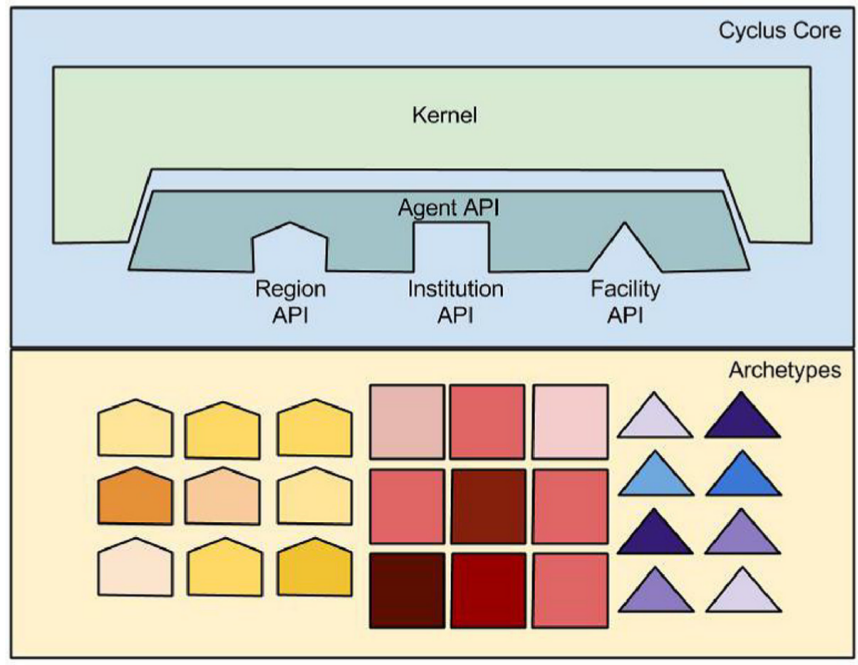
\includegraphics[width=\textwidth]{cyclus_core.png}
    \end{center}
    \caption{The \Cyclus core provides APIs that the archetypes
            can be loaded into the simulation modularly
            \cite{huff_fundamental_2016}.}
    \label{fig:core}
\end{figure}

Due to this modularity in the \Cyclus framework, the developed
model in this work can be implemented independently without
having to modify the \Cyclus source code. The new facility archetype
is simply written with the \Cyclus API, and imported in a
\Cyclus simulation.

\subsubsection{\Cycamore Recipe Reactor}
\Cycamore is a library that consists of useful
fuel cycle facility archetypes for \Cyclus. The
recipe reactor in \Cycamore is a batch-wise reactor.
A reactor core is consisted of multiple batches,
and a batch is consisted of multiple assemblies.
At startup, the reactor requests the entire core,
which is consisted of user-defined number of assemblies.
At every cycle, the reactor discharges and
requests batches of fuel. Upon decommissioning,
the reactor discharges all its fuel. The discharged
fuel is transmutated to the user-defined recipe.
No depletion calculation is performed. However,
the user can define multiple recipes, and can define
times to change the recipe from one to another.

\section{Method}

This work follows four steps:

\begin{enumerate}
\item Data curation
\item Model training (with hyperparameter optimization)
\item Model validation
\item Model implementation in \Cyclus.
\end{enumerate}


First, we curated the
data with assembly information for ease of use in training the model.
Second, we trained the neural network using Keras \cite{collet_keras_2015}
and Scikit-learn \cite{pedregosa_scikit-learn_2011},
while using an outer loop to
search for the optimized set of neural network hyperparameters,
such as the number of hidden layers and nodes per layer.
Third, we used the model to predict the U.S. \gls{UNF}
inventory as specified in the \gls{UDB} and compare
\gls{UNF} inventory metrics such as fissile content
and decay heat. Lastly, we implemented the trained
model in \Cyclus by developing a reactor facility archetype
that transmutes fuel using the model.

The files used to generate and test the neural network
model are all on Github (https://github.com/jbae11/depletion\_rom)
including the pickled neural network model file. The raw data
is not available to the public.

\subsection{Training set}

In order to train a artificial neural network model, a significant database of
depletion data is needed, that span the potential
burnup and enrichment range in typical reactors.

Data from the \gls{UDB} was used to train the model 
based on burnup and enrichment. 

Ideally, the data should be generated with exact same reactor
parameters other than burnup and enrichment, such as geometry or
coolant density. Also, it should be noted that the reactor
parameters could be input values to the neural network model. However, since
this is preliminary work to prove potential workflow, we
simply used all the \gls{PWR} datasets in the \gls{UDB},
and the input values are only burnup and initial enrichment.

\subsubsection{Unified Database}
The \gls{UDB} is part of a larger engineering
analysis tool, the \gls{UNF-STANDARDS}, developed
by \gls{ORNL} \cite{peterson_used_2013}.  
The database provides a comprehensive, controlled
source of \gls{SNF} information, including
dry cask attributes, assembly data, economic attributes,
transportation infrastructure attributes, potential future
facility attributes, and federal government radioactive
waste attributes. 
The assembly-specific attributes include
initial enrichment, burnup, \gls{MTHM}, assembly 
type and discharge date \cite{peterson_fuel_2015}. 
To generate this database, the authors used
irradiation and decay calculations using SCALE 
\cite{bowman_scale_2011}. The calulations were performed on each 
spent fuel assembly based on the previously mentioned 
parameters in the collected data to obtain mass, heat 
and activity for each assembly \cite{peterson_additional_2017}. 
All the assemblies were modeled with conservative 
depletion parameters which result in the hardening of 
the neutron energy spectrum and an increased \gls{SNF} 
residual reactivity \cite{peterson_additional_2017}. 

Also, the irradiation history of the fuel is unspecified in the
database, which can be a source of deviation for short-lived isotopes.
With the unknown parameters (unknown irradiation history, variyng
assembly models) and assumptions (conservative composition to
increase fuel reactivity), the database is far from ideal to use
as a training dataset for a depletion calculation model. However,
we chose this data set because it allows testing of model performance
through comparision of \gls{UNF}
inventory between a high-fidelity model and a model prediction for
varying burnup, enrichment, and discharge time.

Ideally, the data should be generated with exact same reactor
parameters other than burnup and enrichment, such as geometry or
coolant density. However, since
this is preliminary work to prove potential workflow, we
simply used all the \gls{PWR} datasets in the \gls{UDB}.

We received the database through personal contact with
Kaushik Banerjee, one of the original creators of the database.
The database is currently accessible via \gls{RSICC}.

\subsection{Data Curation}

We curated the raw \gls{UDB} datasets to generate
a cleaner training set. First we only used the 
\gls{PWR} assemblies since \gls{BWR} \gls{UNF} assembly
calculation results can vary significantly with void fraction.
We also filtered out the
`very low' enrichment ($\leq$ 1.5) and
burnup ($\leq$ 10,000 MWd/MT)
assemblies to represent a more modern \gls{PWR} \gls{UNF}
assembly range. Figure \ref{fig:enr_bu} shows the
burnup and enrichment distribution of the assemblies in the
\gls{UDB}.


\begin{figure}
    \centering
    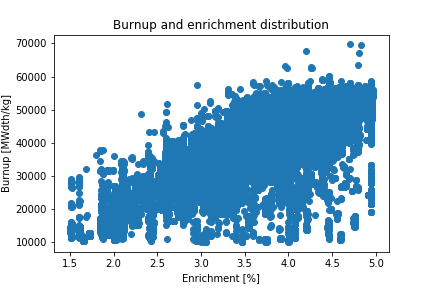
\includegraphics[width=\textwidth]{enr_bu.png}
    \caption{Burnup and enrichment distribution of train
             datasets curated from the \gls{UDB}.}
    \label{fig:enr_bu}
\end{figure}


Also, the SCALE calculation in the \gls{UDB} only tracks 60 isotopes
and on average 3.5 weight percent of the \gls{UNF} is not accounted for. We
aggregate the isotopes not accounted for as a separate category. Lastly,
we processed the database so that the isotopic compositions are 
represented as weight \% from initial uranium mass, to normalize
the dataset. For every isotope \textit{i}:

\begin{equation}
x_i = \frac{m_i}{M_{initU}}
\end{equation}
where:
\[
x_i = \text{\% weight of isotope in depleted assembly}
\]
\[
m_i = \text{mass of isotope in depleted assembly in \gls{UDB}}
\]
\[
M_{ITHM} = \text{Mass of initial uranium in assembly}
\]


\subsection{Predictive Models for Fuel Depletion}

\gls{UNF} depleted composition is difficult to predict
due to the varying relationship with the fuel parameters.
In figures \ref{fig:cs_137, fig:pu_239, fig:u_235},
we plotted isotopic concentration values against
burnup and enrichment, to observe the relationship between
burnup, enrichment, and isotopic concentration.

We observed that the isotopic concentration has varying
relationships with fuel burnup and enrichment.
For example, if the isotopic population is mainly determined by
the fission of initial uranium, a linear regression algorithm
can be used to predict the isotopic concentration from burnup
(Cs-137 shown in figure \ref{fig:cs_137}).
However, isotopes like plutonium-239 (figure \ref{fig:pu_239}) have multiple, conflicting creation
and destruction terms, making it harder to predict using a
linear regression algorithm. Also, the uranium-235 (figure \ref{fig:u_235}) concentration
depends on both burnup and enrichment, which can make it
hard to predict using a simple linear model.

Due to these complexities, we decided to train an artificial
neural network for our predictive model. We chose
Keras \cite{collet_keras_2015} to create and validate the model,
as well as scikit-learn \cite{pedregosa_scikit-learn_2011}
and pandas \cite{mckinney-proc-scipy-2010} for data processing and management.

\begin{figure}
    \centering
    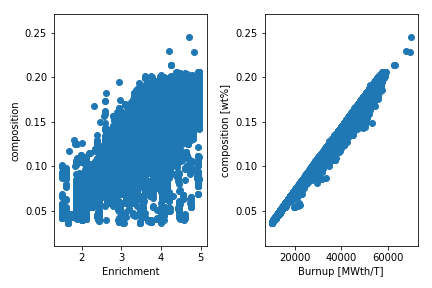
\includegraphics[width=\textwidth]{cs-137_sub.png}
    \caption{$^{137}Cs$ concentration in a \gls{UNF} assembly
             varies linearly with assembly burnup.}
    \label{fig:cs_137}
\end{figure}

\begin{figure}
    \centering
    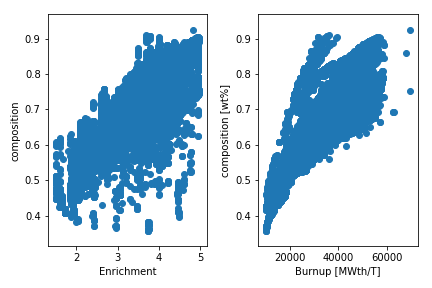
\includegraphics[width=\textwidth]{pu-239_sub.png}
    \caption{$^{239}Pu$ concentration in a \gls{UNF} assembly
             is not linearly related to burnup, since it
             is affectex by multiple, conflicting creation
             and destruction terms}
    \label{fig:pu_239}
\end{figure}


\begin{figure}
    \centering
    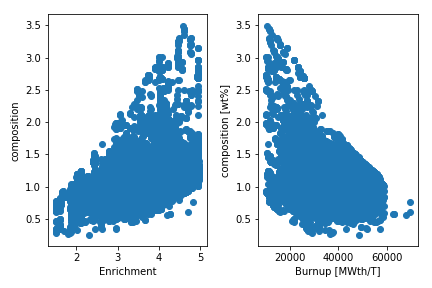
\includegraphics[width=\textwidth]{u-235_sub.png}
    \caption{$^{235}U$ concentration in a \gls{UNF} assembly
             somewhat proportional to both enrichment and
             burnup, but is difficult to predict using
             a simple linear regression algorithm.}
    \label{fig:u_235}
\end{figure}


\subsection{Training and Selecting Models}

The inputs (features) of the model are
burnup (MWd/MT) and initial enrichment (wt\% $^{235}U$).
The outputs (targets) of the model are
the concentration (weight \%) of the 60 isotopes in the
depleted assembly.

With the curated dataset, we performed an outer loop
search to find the best-performing neural network
hyperparameter. First, we set 20 percent of the 
data for final model testing purpose. We used a three-fold
cross validation \cite{stone1974cross} on the remaining
dataset, to
measure the average prediction error value. We
normalized the data using the sklearn MinMaxScaler
so that the range of input and output data is (0,1).

\begin{table}[h]
    \centering
    \begin{tabular}{lr}
        \hline
        Parameter & Values \\
        \hline
        Number of hidden layers & 1, \textbf{2}, 3, 4 \\
        Nodes per hidden layer & 4, 16, 32, 64, \textbf{128} \\
        Dropout rate & \textbf{0.0}, 0.2, 0.5 \\
        \hline
    \end{tabular}
    \caption{Table of hyperparameters tested
             for neural network model. The bold
             numbers are the values we used for the final model.}
\end{table}


We selected the model with the smallest average error value
and exported the model as a file using python
pickle file, along with the dataset normalization objects, and 
the list of isotopes. By exporting the trained model
as a self-contained file, the model can be used in any python
application.


\subsection{Model Testing}

We tested the accuracy of the model by comparing
the model's \gls{UNF} composition prediction
in three different cases. First, we compared the
isotope-by-isotope prediction error of the model for an
assembly with a specific burnup and enrichment.
Second, we compared the waste characteristics of
an assembly for all assemblies. Third, we compared
the predicted total \gls{PWR} \gls{UNF} inventory with
\gls{UDB}. The metric for error is calculated as
relative error percentage, calculated by:
\begin{equation}
\epsilon = \frac{x_{data} - x_{model}}{x_{data}}
\end{equation}

This metric is to provide a fair assessment to errors
in predicting isotopes with minute concentration in \gls{UNF}.
However, it should be noted that a large error percentage in the
prediction of these minute isotopes is mostly because it has been
divided by a small value, not because the absolute error is large.

We compared parameters of the \gls{UNF} inventory
such as activity and decay heat, using the
\gls{PyNE} \cite{scopatz_pyne:_2012}. This tool provides
various functions used
in this work, such as decaying and calculating
the activity and decay heat of the \gls{UNF} inventories.

Ideally, the model should be tested against data
that is not part of the training data. However, given
that the purpose of this model is to allow accessible and
quick depletion calculation for
fuel cycle simulations, the model would suffice if
it predicts the dataset well. In other words, the
goal of the model is to be able to reproduce,
in a continuous manner, the range of fuel depletion
calculations in the database without access to the particular dataset.
This work
is to propose a general concept for implementing
rapid depletion models in fuel cycle simulations.
For creating depletion models for other reactor designs or depletion parameters,
one would simply change the dataset to a set of depletion calculations performed
for a specific reactor design and operational parameters.

We also tested the neural network's performance with the
test set that was set aside prior to the hyperparameter search.



\subsection{Model Implementation in \Cyclus}

The trained model is exported to a file
that can be plugged into external codes. \Cyclus
has a python interface that allows the developer
to design archetypes in python. We developed a reactor
module that behaves similarly to the recipe reactor
but calculates depleted fuel concentration using the
imported model instead of a recipe. The user can vary
individual assembly burnups. The user defines a burnup
and enrichment
matrix for the reactor. The rows are the number
of batches, and the columns are the number of
assemblies in a batch. This reactor module is also
available on Github 
(https://github.com/jbae11/ann\_pwr).

This sort of implementation can be done with
a recipe-based approach for modeling reactor depletion
if the user defines multiple
output recipes. However, the user can only define
the recipe of a batch.
Implementing this trained neural network model will allow the user to vary
burnup and enrichment for individual assemblies, as well
as vary fuel residence time and burnup with reactor
lifetime or simulation time. Such capability will be
useful in simulating \gls{UNF} inventory in the future,
where the burnup of \gls{LWR} fuel will increase
with advanced fuel technology.
\section{Results}

The model performed better than using the average
recipe in predicting the U.S. \gls{UNF}, with
negligible increase in computational time.

\subsection{Depletion Calculation Time and File Size}
For 100 random sets of
burnup and enrichment depletion predictions,
the model takes 0.27 seconds to output discharge composition, while
searching the database for assemblies
with the closest burnup and enrichment (using Pandas)
takes 21.8 seconds. Comparatively, 100 \gls{ORIGEN} calculations
take 118 seconds. Using the model achieves 43,700\% reduction
in time and does not require libraries, or reactor physics code.
The standalone model pickle file is only
38 Kb, while the curated database (.csv) itself is 330 Mb.

\subsection{Assembly Comparison}

Ten data points were randomly sampled from the \gls{UDB},
and were compared with the model predictions to observe
two things:
\begin{enumerate}
    \item What isotopes the model is good / bad
        at predicting
    \item What burnup / enrichment range the model is good / bad
        at predicting
\end{enumerate}

Figures \ref{fig:3-2_29998-0}, \ref{fig:3-81_35883-0},
\ref{fig:4-0_35195-0}, and \ref{fig:4-47_50105-0}
show that the model
generally has a high relative error percentage for \textsuperscript{226}Ra
(average concentration $6.0\times10^{-12}\%$),
\textsuperscript{227}Ac (average concentration  $2.3\times10^{-12}\%$), and curium isotopes.
The absolute prediction errors are quite small
(averaging $1e-11$), but the large percent errors are due
to the small value of the data. There was not a notable
difference in the error values for enrichment
and burnup variations.

\begin{figure}
    \centering
    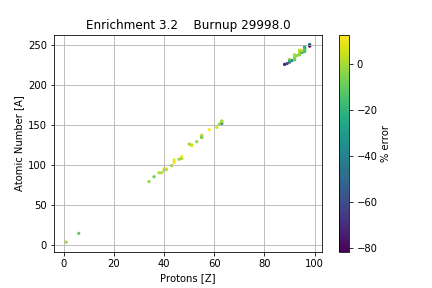
\includegraphics[width=\textwidth]{3-2_29998-0.png}
    \caption{Isotopic composition prediction error for an assembly with 
             $29.998 \frac{GWd}{MT}$ burnup and 3.2  \% enrichment.}
    \label{fig:3-2_29998-0}
\end{figure}

\begin{figure}
    \centering
    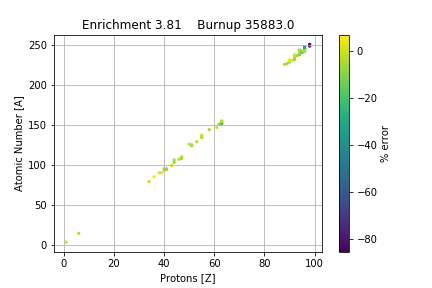
\includegraphics[width=\textwidth]{3-81_35883-0.png}
    \caption{Isotopic composition prediction error for an assembly with 
             $35.883 \frac{GWd}{MT}$ burnup and 3.81  \% enrichment.}
    \label{fig:3-81_35883-0}
\end{figure}

\begin{figure}
    \centering
    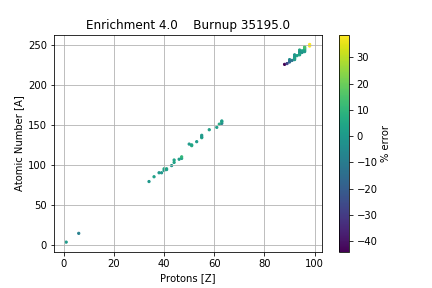
\includegraphics[width=\textwidth]{4-0_35195-0.png}
    \caption{Isotopic composition prediction error for an assembly with 
             $35.193 \frac{GWd}{MT}$ burnup and 4.0 \% enrichment.}
    \label{fig:4-0_35195-0}
\end{figure}


\begin{figure}
    \centering
    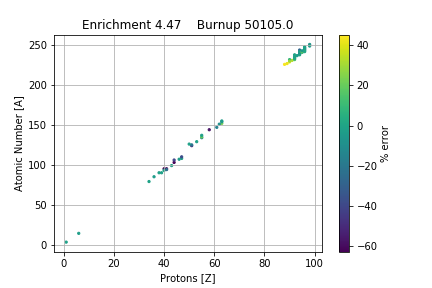
\includegraphics[width=\textwidth]{4-47_50105-0.png}
    \caption{Isotopic composition prediction error for an assembly with 
             $50.105 {GWd}{MT}$ burnup and 4.47  \% enrichment.}
    \label{fig:4-47_50105-0}
\end{figure}

\FloatBarrier

\subsection{U.S. \gls{UNF} Inventory Comparison}

In this section, we compare three \gls{UNF} inventory composition
model approaches.
The only difference is the composition of the
assemblies. The three different inventory compositions were acquired by:

\begin{enumerate}
    \item \textbf{Data}: directly query the assembly composition from the \gls{UDB}.
    \item \textbf{Prediction}: neural network prediction of depleted composition using burnup and enrichment from database
    \item \textbf{Recipe}: using a single composition (recipe) for all assemblies. Assumes all compositions are the same.
\end{enumerate}

The median values for burnup and initial enrichment are
$41,552$ MWd/MT and 3.85 (wt\%), respectively. The concentrations of major
isotopes in the assembly are in Table \ref{tab:avg_assem}.


\begin{table}[h]
    \centering
    \begin{tabular}{|l|r|r|r|r|r|}
        \hline
        Isotopes & $^{235}U$ & $^{238}U$ & $^{239}Pu$ & $^{137}Cs$ & $^{90}Sr$ \\
        \hline
        Concentration [wt\%] & 1.076 & 92.66 & 0.77 & 0.14 & 0.061 \\
        \hline
    \end{tabular}
    \caption{Isotopic concentration of the assembly with median burnup and
             enrichment. This composition is used for the recipe method. 
    \label{tab:avg_assem}}
\end{table}


We compare the three composition predictions according to:
\begin{enumerate}
    \item Isotopic inventory
    \item Waste metrics (activity and decay heat)
    \item Equivalent fissile inventory (equivalent $^{239}Pu$)
\end{enumerate}

The \gls{UDB} contains discharged assembly data
from nuclear reactors in the United States up to May of
2013. We added all the \gls{UNF} assemblies in the database,
and evaluated the inventory as it was in 2013. 
Table \ref{tab:met} shows the comparison of the inventories.

\begin{table}[h]
    \centering
    \begin{tabular}{l|r|rr}
        \hline
        Metric & Data & Recipe & Prediction \\
        \hline
        $^{239}Pu$ mass [t] & 320.37 & 351.70 & 321.38\\
        $^{137}Cs$ mass [t] & 63.84 & 66.64 & 63.73 \\
        $^{235}U$ mass [t] & 464.60 & 487.94 & 474.14\\
        $^{238}U$ mass [t] & 42,171 & 42,016 & 42,162\\
        \hline
        Decay Heat [MW] & 193.39 & 198.55 & 193.33 \\
        Activity [$E+21$Bq] & $2.79$ & $2.84$ & $2.75$ \\
        \hline
    \end{tabular}
    \caption{Comparison of \gls{PWR} \gls{UNF} inventory in the U.S,
             obtained from direct data query, recipe approach,
             and neural network prediction. 
    \label{tab:met}}
\end{table}

\FloatBarrier

\subsubsection{Isotopic Inventory}

In terms of isotopic composition accuracy, the trained
neural network model outperforms the
mean recipe method for all isotopes.
Figure \ref{fig:iso_rel} shows the relative
error between the full database, model prediction, and
the mean recipe for
major isotopes. For plutonium isotopes, the trained neural
network model far
outperforms the mean database.

\begin{figure}
    \centering
    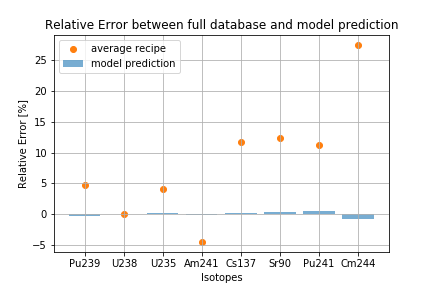
\includegraphics[width=\textwidth]{iso_rel.png}
    \caption{Neural network model prediction error relative to median
             \gls{UDB} recipe, for key isotopes.}
    \label{fig:iso_rel}
\end{figure}


\begin{figure}
    \centering
    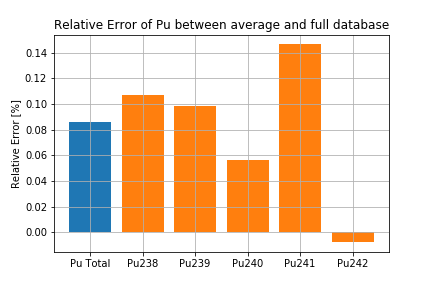
\includegraphics[width=\textwidth]{pu_rel.png}
    \caption{Neural network model prediction error relative to median
             \gls{UDB} recipe, for plutonium isotopes.}
    \label{fig:pu_rel}
\end{figure}

\FloatBarrier


\subsubsection{Waste Management Metrics}
The trained neural network excellently predicts the activity
and decay heat metrics. Figures \ref{fig:assem_dh} and \ref{fig:assem_act}
show the relative error percent of the decay heat and activity
predictions per assembly. The model predicts 99.5\% of
assemblies with an error of less than 1\%.
Figures \ref{fig:assem_dh_recipe} and
\ref{fig:assem_act_recipe} show the relative error
of the decay heat and activity calculated with the average
recipe method.
Unsurprisingly, the error increases as the actual burnup and enrichments
diverge from the average.

\begin{figure}
    \centering
    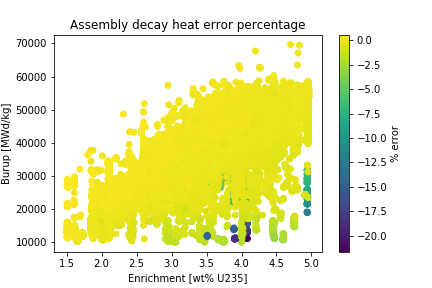
\includegraphics[width=\textwidth]{assem_dh.png}
    \caption{Relative error percentage for predicting the decay
             heat of individual assemblies.}
    \label{fig:assem_dh}
\end{figure}


\begin{figure}
    \centering
    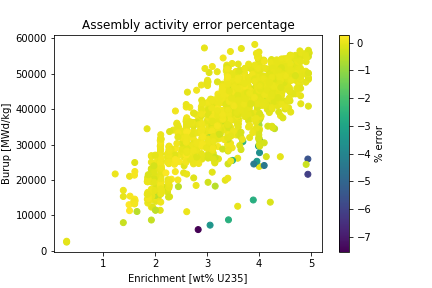
\includegraphics[width=\textwidth]{assem_act.png}
    \caption{Relative error percentage for predicting the
             activity of individual assemblies.}
    \label{fig:assem_act}
\end{figure}



\begin{figure}
    \centering
    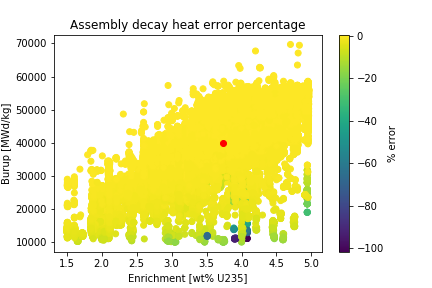
\includegraphics[width=\textwidth]{assem_dh_recipe.png}
    \caption{Relative error in decay heat calculated by the average recipe
             method. The red point is the median enrichment and
             burnup.}
    \label{fig:assem_dh_recipe}
\end{figure}

\begin{figure}
    \centering
    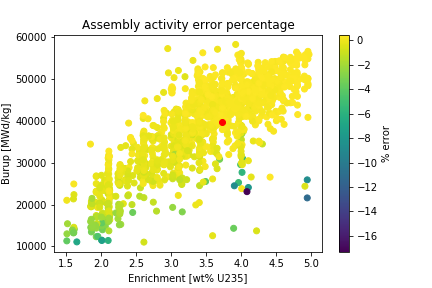
\includegraphics[width=\textwidth]{assem_act_recipe.png}
    \caption{Relative error in activity
             calculated by the average recipe method.
             The red point is the median enrichment and
             burnup.}
    \label{fig:assem_act_recipe}
\end{figure}

\FloatBarrier


Table \ref{tab:wm} shows the decay heat and activity
comparison in the years 2020, 2100, and 3100. The total
error is less than 1.1\% for all metrics at all time periods.
Figure \ref{fig:ha_err} shows relative error in activity and
decay heat as a function of time. It shows
that the model outperforms the average recipe method
in predicting waste metrics.

%! Do the decimal centering
\begin{table}[h]
    \centering
    \begin{tabular}{lcrrr}
        \hline
        Metric & Year & UDB [MW] & Prediction [MW]  & Error [\%] \\
        \hline
        \multirow{3}{*}{\shortstack{Decay \\ Heat }} & 2020 & 40.97 & 41.07 & -0.24 \\
                                                    & 2100 & 16.42 & 16.47 & -0.35 \\
                                                    & 3100 & 3.13 & 3.14 & -0.15 \\
        \hline
         & & UDB [$10^{19}$Bq] & Prediction [$10^{19}$Bq] & Error[\%] \\
        \multirow{3}{*}{\shortstack{Activity}} & 2020 & 46.70 & 46.60 & 0.21 \\
                                               & 2100 & 6.39& 6.38 & 0.07 \\
                                               & 3100 & 0.36 & 0.36 & -0.17 \\
        \hline
    \end{tabular}
    \caption{Decay heat and radioactivity values and errors for years 2020, 2100, and 3100.}
    \label{tab:wm}
\end{table}

\begin{figure}
    \centering
    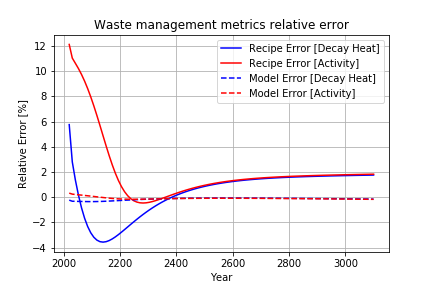
\includegraphics[width=\textwidth]{ha_err.png}
    \caption{Relative error of waste management metrics for \gls{UNF} inventory
             generated by the average recipe and the prediction model.}
    \label{fig:ha_err}
\end{figure}

\FloatBarrier

\subsubsection{Assembly fissile quality}

Fissile quality is frequently quantified in units of 
$^{239}Pu$ equivalent, shown in figure \ref{tab:pu_equiv} \cite{anon_plutonium_1989}. This value is
calculated by aggregating the weighted fissile
values of each isotope in a material. The $^{239}Pu$
equivalent factors are different for fast neutron spectrum 
and thermal neutron spectrum reactors \cite{baker_comparison_1963}.  
For example, the equivalent fissile value for
an \gls{LWR} will be calculated by:
\begin{gather*}
\text{Pu}_{\text{eq}} = \sum_i w_i m_i \\
i \in [^{235}U, ^{238}Pu, ^{239}Pu, ^{240}Pu, ^{241}Pu, ^{242}Pu, ^{242}Am] \\
w_i = \text{equivalent weighting factors} \\
m_i = \text{mass of iso i} \\
\end{gather*}
Where the variables represent the mass of each isotope.



\begin{table}[h]
    \centering
    \begin{tabular}{ccc}
        \hline
        & \multirow{2}{*}{\shortstack{LWR \\ (Thermal)}} &
        \multirow{2}{*}{\shortstack{\gls{FBR}\\ (Fast)}} \\ \\
        \hline
        $^{235}U$ & +0.8& +0.8\\
        $^{238}Pu$ & -1.0& +0.44\\
        $^{239}Pu$ & +1.0& +1.0\\
        $^{240}Pu$ & -0.4& +0.14\\
        $^{241}Pu$ & +1.3& +1.5 \\
        $^{242}Pu$ & -1.4& +0.037\\
        $^{241}Am$ & -2.2& -0.33\\
        \hline
    \end{tabular}
    \caption{$^{239}Pu$ equivalence factors from \cite{anon_plutonium_1989}.
             Factors are separately reported for thermal and fast spectra.}
    \label{tab:pu_equiv}
\end{table}


Figure \ref{fig:fiss} shows the fast spectrum $^{239}Pu$ equivalent
value of the \gls{UNF} inventory plotted over time.
The trained model outperforms the recipe method. The
initial falls for all three lines are due to the
decay of plutonium 241, which has a half-life of
14 years.


\begin{figure}
    \centering
    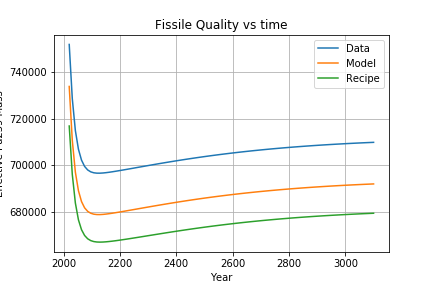
\includegraphics[width=\textwidth]{fiss.png}
    \caption{$^{239}Pu$ equivalent value in time for three
             inventories. The model predictions match closely
             with the value from the database.}
    \label{fig:fiss}
\end{figure}




\subsection{\Cyclus implementation}

In this work, we trained a neural
network model and implemented it as a  \Cyclus reactor
agent that predicts \gls{UNF} composition. The model predicts spent
fuel composition
based on customizable reactor parameters such as
discharge burnup, initial enrichment, cycle time, and power
capacity. The created archetype in \Cyclus also allows users to define
time-dependent
equations instead of constants for reactor parameters.
The user can define an enrichment-burnup matrix for
each assembly in each batch, and the burnup and enrichment
values can be equations in time. This way, users can
implement reactor facilities in which the reactor parameters
change in time (e.g. to represent reactor uprates, industry
burnup trends, etc.).

Figures \ref{fig:cyclus_pu}
and \ref{fig:cyclus_fp} show the discharge fuel composition
of a reactor facility in which we increased the discharge burnup
from 33,000 to 71,710 MWd/MT over 25 discharge cycles.
It should be noted that the model does not take into account
the plausibility of such fuel depletion. For example, it
would be nearly impossible for a  \gls{PWR} to burn 2\%
enriched \gls{UOX} fuel to 70,000 MWd/MT.

The user can also define time-varying
cycle time and refueling time for the reactor model, as shown
in figure \ref{fig:cyclus_time}.


%! it is plutonium in the fuel total
\begin{figure}
    \centering
    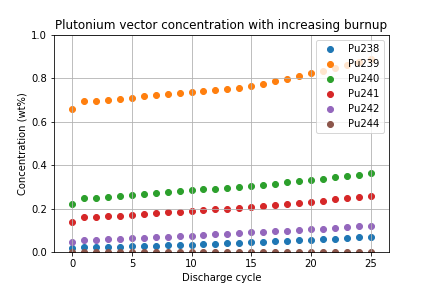
\includegraphics[width=\textwidth]{./cyclus_imp/pu.png}
    \caption{Plutonium isotope composition in discharge fuel over discharge cycle. The model does not predict well for the target burnup values
    that are over the burnup listed in the training dataset.}
    \label{fig:cyclus_pu}
\end{figure}


\begin{figure}
    \centering
    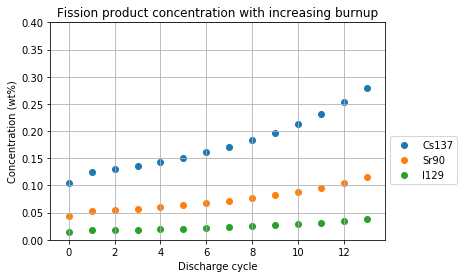
\includegraphics[width=\textwidth]{./cyclus_imp/fp.png}
    \caption{Fission product concentration in discharge fuel over discharge cycle. Increased discharge burnup leads to higher fission product concentration.}
    \label{fig:cyclus_fp}
\end{figure}


\begin{figure}
    \centering
    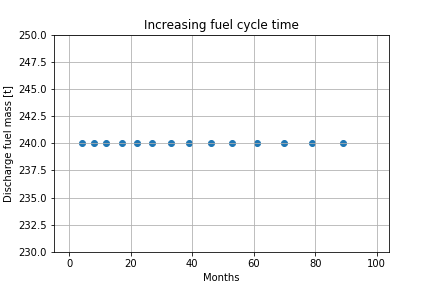
\includegraphics[width=\textwidth]{./cyclus_imp/cycle_time.png}
    \caption{Discharge and refueling cycles can be defined as an equation of time in this reactor archetype. Discharge burnup is scaled to take into account longer fuel residence time, and leads to increase in discharge fuel \textsuperscript{244}Cm composition.
    }
    \label{fig:cyclus_time}
\end{figure}

\subsubsection{Applications and Use Cases}

The capability to set dynamic reactor parameters
allows simulation of various future transition scenarios
that depend on \gls{UNF} inventory characteristics,
such as \gls{MA} inventory. 
Users can simulate future scenarios in which the discharge
burnup of reactors increases over time to reveal
impacts on \gls{MA} inventory and, correspondingly,
transition speed. 

With
advances in materials, reactors may have longer
cycle times and higher fuel discharge burnups.
This dynamic reactor model will be able to account
for the changes in these reactor parameters.
Also, users can simulate potential
power uprates in currently existing fleets, and
estimate corresponding impacts on \gls{UNF} inventory.
\FloatBarrier
\section{Conclusion and Discussion}

This work shows that depleted fuel composition
in fuel cycle simulators can be improved
by using a neural network predictive model.
The neural network model predicted the \gls{UNF} inventory
with less than 5\% error for individual isotopes,
less than 1\% error for waste profile 
and less than 0.1\% error for the fissile quality.
The predictive model outperformed the average recipe
method in every metric.

We implemented this model in \Cyclus to develop a
dynamic reactor model with changing reactor parameters,
which can simulate potential future improvement scenarios
in reactor operation.

This work also shows that quick, open-source depletion models
can be implemented using prediction models, from
complex, inaccessible depletion algorithms and
datasets. \gls{NFC} simulators struggle to find a balance
between fidelity and rapidity. Using high-fidelity
models become prohibitively computationally expensive
since \gls{NFC} simulators may need to run
hundreds of depletion calculations for multiple
facilities. On the other hand, using simpler methods
like recipes are overly simplified solutions
that do not take into account variations in fuel
parameters such as burnup.
A well-trained predictive algorithm can find a middle
ground between rapidity and fidelity.

We cannot avoid the criticism that the model is validated
against the dataset used to train the model. However, the purpose
of this work is to create a model that can quickly reproduce the
database without having access to the database, which is proprietary
and large in size. The pickled file that contains
the model and data scaling objects is only 38.2 kB, meaning that it
can be easily distributed and imported in external software, without
revealing any information on the actual proprietary dataset.

[cringe]

It is noteworthy that there are not a lot of accessible data in the
nuclear engineering discipline. Large-scale depletion
calculation results like the \gls{UDB} are exceptional
but rare cases. The value of data is exponentially increasing,
with the advancement of data science and machine learning.
For the long-term advancement of the field, maybe the
community should encourage collection and storage of more
data and simulation results in
a central repository, for the betterment of the field.

[cringeend]


\section{Future Work}

A trained model is only as good as the data it is trained on.
This work can be improved and expanded by generating
more comprehensive depletion data that covers a wider
range of enrichment and burnup ranges. An automation
script might run SCALE ORIGEN to perform depletion calculations
for a wide range of enrichment (e.g. 0.7 - 4.99 wt\%) and burnup (e.g. 0 - 80,000 MWd/MT),
for a single assembly design. Assumptions of criticality
and irradiation time should be made as well. The results
could then be parsed into a \gls{CSV} file and stored for
the training of a new model. This will allow better
prediction of the model for higher burnups and `fringe'
burnup-enrichment assemblies.

Methods used in this paper have the potential to be expanded into more
complicated problems. For example, the method
could be applied to \gls{MOX} fuel depletion, taking
into account varying uranium and plutonium concentrations.
However, a \gls{UDB} equivalent is not available
for training a \gls{MOX} model, so a
data-generating process, consisting of a high-fidelity
depletion calculation of randomized \gls{MOX} fuel
compositions within acceptable ranges of reactor
criticality, similar to the process mentioned above,
will have to take place. After the data
is generated, the neural network model can be trained
to predict \gls{MOX} depletion.

Another interesting application of this method is for
\gls{MSR} system optimization. Current work on
\glspl{MSR} include optimization non-core operating
parameters such as reprocessing scheme and flow rate.
Fuel transmutation calculations
can be usually computationally burdensome for \gls{MSR}
simulations, since the flowing fuel is depleted and
reprocessed continuously. \gls{MSR} models implement semi-continuous
methods in which the depletion-to-reprocessing time is
very short (usually 3 days), which makes an
\gls{MSR} lifetime simulation (if 60 years)
require $\sim 7,300$ depletion calculations.
The computational burden
makes it impossible to use brute-force methods,
such as grid search of all possible parameters.
However, if a quick depletion calculation becomes possible
with a well-trained prediction model, the
computational burden will dramatically decrease.
However, problems with generating enough
training data, accuracy, and the model's ability to
extrapolate remain.

\pagebreak
\section{References}
\bibliography{bibliography}


\end{document}
